\documentclass[12pt, a4paper]{article}
\usepackage[utf8]{inputenc}
\usepackage[spanish]{babel}
\usepackage[table]{xcolor}
\usepackage{url, hyperref}
\usepackage{graphicx, listings, xcolor, adjustbox, caption, subcaption, float, amsmath}

\definecolor{codegreen}{rgb}{0,0.6,0}
\definecolor{codegray}{rgb}{0.5,0.5,0.5}
\definecolor{codepurple}{rgb}{0.58,0,0.82}
\definecolor{backcolour}{rgb}{0.95,0.95,0.92}

\lstdefinestyle{mystyle}{
    backgroundcolor=\color{backcolour},   
    commentstyle=\color{codegreen},
    keywordstyle=\color{magenta},
    numberstyle=\tiny\color{codegray},
    stringstyle=\color{codepurple},
    basicstyle=\ttfamily\footnotesize,
    breakatwhitespace=false,         
    breaklines=true,                 
    captionpos=b,                    
    keepspaces=true,                 
    numbers=left,                    
    numbersep=5pt,                  
    showspaces=false,                
    showstringspaces=false,
    showtabs=false,                  
    tabsize=2
}

\setlength{\parindent}{0pt}
\setlength{\parskip}{12pt}
\renewcommand{\arraystretch}{1.5}
\lstset{style=mystyle, language=c++}

\title{\vspace{-3cm}Examen Parcial 1: Problema Knapsac con ACO}
\author{
    Universidad Autónoma de San Luis Potosí\\ 
    Facultad de Ingeniería - Ing. en Sistemas Inteligentes\\ 
    \textbf{Materia:} Cómputo Bioinspirado \\
    \textbf{Prof:} Dr. Cesar Augusto Puente Montejano  \\
    \textbf{Autor:} Angel de Jesús Maldonado Juárez
}
\date{\textbf{Fecha de entrega:} viernes 23 de septiembre de 2022}

\begin{document}

\maketitle

\section{Planteamiento del Problema}\label{title1}
El problema a resolver tiene el siguiente enunciado:

Un ladrón llega a robar a una casa. Para su buena suerte, encuentra un salón lleno de objetos
sumamente valiosos. Para su mala suerte, solo lleva una pequeña mochila que puede soportar cuando
mucho 10 kilogramos de peso. Por lo tanto, debe decidir qué objetos puede cargar, tratando de
llevarse la mayor ganancia posible. Entre los objetos que encontró están los siguientes:

\begin{table}[!ht]
    \begin{adjustbox}{width=\textwidth}
        \begin{tabular}{|c|c|c|c|c|c|c|c|}
            \rowcolor{yellow}
            \hline
                  & Centenarios & Billetes de 1000 & Joyero (gde) & Joyero (ch) & Estampillas & Obra de arte & Pisapapeles de oro \\
            \hline
            Valor & \$750,000   & \$500,000        & \$2,750,000  & \$950,000   & \$1,850,000 & \$3,250,000  & \$3,950,000        \\
            \hline
            Peso  & 2.5         & 1                & 6            & 2.5         & 1.5         & 3            & 5                  \\
            \hline
        \end{tabular}
    \end{adjustbox}
\end{table}

¿Cuáles objetos se debería llevar si quiere conseguir la mayor cantidad de dinero sin sobrepasar el
peso de la mochila?

\section{Descripción de la Solución}
Con base en la implementación (en C++) encontrada \cite{qcloud1223_2022}, se puede representar el espacio del problema como un \textbf{completamente conectado}, en el cual los \emph{nodos} representan los objetos que el ladrón puede urtar:

\begin{figure}
    \centering
    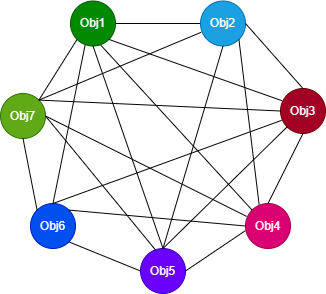
\includegraphics[width=0.4\textwidth]{img/grafo.png}
    \caption{Representación del problema en un grafo}
\end{figure}

Debido a que cada nodo (objeto) tiene 2 parámetros que definen la \emph{deseabilidad} del mismo, la matriz $\eta$, que representaría la matriz de costos de las aristas, se simplifica a un único vector de tamaño del número de objetos ($7$), y en cada posición se almacena: $\frac{valor del objeto}{peso del objeto}$, teniendo así un vector heurístico que engloba tanto el valor monetario del objeto como el peso del objeto. La matriz de feromonas $\tau$ también se simplifica a un vector de tamaño del número de objetos iniciando todos los valores en $1$.

Finalmente, una de las limitaciones más importantes de esta implementación, es que las dimensiones de la matriz de movimiento de las hormigas se define como $(NumHormigas,NumObjetos)$, y para abarcar la mayor cantidad de posibilidades, cada hormiga $i$ parte desde la posición $(i,i)$, esto implica que $NumHormigas$ no puede ser mayor a $NumObjetos$, teniendo la \emph{máxima} matriz de movimiento con $NumHormigas=NumObjetos$:

\begin{equation}
    \begin{bmatrix}
        1 & 0 & 0 & 0 & 0 & 0 & 0 \\
        0 & 1 & 0 & 0 & 0 & 0 & 0 \\
        0 & 0 & 1 & 0 & 0 & 0 & 0 \\
        0 & 0 & 0 & 1 & 0 & 0 & 0 \\
        0 & 0 & 0 & 0 & 1 & 0 & 0 \\
        0 & 0 & 0 & 0 & 0 & 1 & 0 \\
        0 & 0 & 0 & 0 & 0 & 0 & 1 \\
    \end{bmatrix}
\end{equation}

En el código de la implementación además de definir los parámetros y matrices del algoritmo ACO ($nHormigas, maxIter, Q, \tau, \alpha, \beta, \rho$), establece un vector \lstinline{curr_weight} de tamaño $nHormigas$ en el cual se irán guardando la sumatoria de los pesos de la combinación de objetos que del mejor resultado de tal sumatoria, además hay otro vector \lstinline{curr_value} que toma en cuenta el costo de los objetos.

La parte \emph{crítica} del algoritmo es cuando se actualiza la posición de las hormigas (movimiento), esto se realiza con la siguiente línea de código:

\begin{lstlisting}
    if(probability[i][j]>rann&&curr_weight[i]>=weight[j])
\end{lstlisting}

En esta línea, además de tomar en cuenta las probabilidades de que una hormiga elija el siguiente objeto a explorar, también evalúa si el peso de tal objeto es menor del que se encuentra actualmente. Si la condición se cumple, entonces el programa simplemente va marcando con $1$ los objetos que las hormigas vayan decidiendo explorar, además de actualizar los vectores \lstinline{curr_weight} y \lstinline{curr_value}:

\begin{lstlisting}
    Move[i][j] = 1;
    tabu[i][j] = 1;
    curr_weight[i] -= weight[j];
    curr_value[i] += value[j];
\end{lstlisting}

Además se agregó el vector \lstinline{objectsExplored} de tamaño $nObjetos$ inicializado en $0$, con tal de marcar con un $1$ aquellos objetos que quedan registrados como explorados durante la ejecución del algoritmo:

\begin{lstlisting}
    // Despues de Move, tabu, curr_weight, y curr_value
    if (objectsExplored[j] != 1)
    {
        objectsExplored[j] = 1;
        if (objectsExplored[i] != 1)
            objectsExplored[i] = 1;
    }
\end{lstlisting}

En vez de que el programa pregunte mediante la consola el tamaño del problema y asignar pesos y costos manualmente se definieron también estos vectores antes de iniciar el algoritmo:

\begin{lstlisting}
    int n = 7;
    float weight[n] = {2.5, 1, 6, 2.5, 1.5, 3, 5};
    float value[n] = {750000, 500000, 2750000, 950000, 1850000, 3250000, 3950000};
\end{lstlisting}

\section{Descripción de Resultados}
A continuación se muestran múltiples resultados arrojados en la consola, el primer arreglo de números representa los objetos que se elijieron (los marcados con 1), y el número de mayor cantidad el costo total maximizado de los objetos que puede cargar el ladrón.

\textbf{alpha=0.7, beta=2.3, iter=1, nAnts=7}
\begin{figure}[!ht]
    \centering
    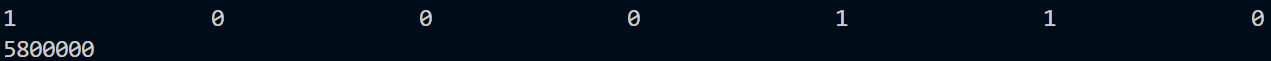
\includegraphics[width=\textwidth]{img/corrida1.png}
\end{figure}

\textbf{alpha=1, beta=2, iter=3, nAnts=7}
\begin{figure}[!ht]
    \centering
    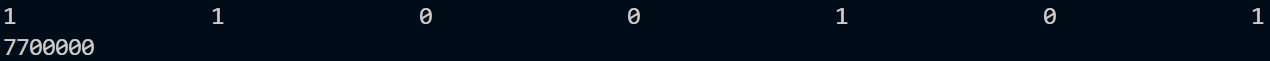
\includegraphics[width=\textwidth]{img/corrida2.png}
\end{figure}

\textbf{alpha=1, beta=2, iter=5, nAnts=7}
\begin{figure}[!ht]
    \centering
    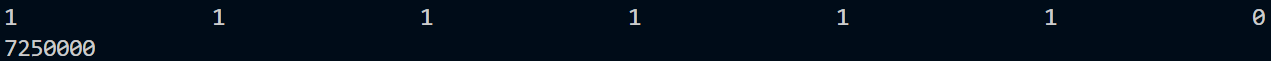
\includegraphics[width=\textwidth]{img/corrida3.png}
\end{figure}

\textbf{alpha=1, beta=2, iter=1000, nAnts=7}
\begin{figure}[!ht]
    \centering
    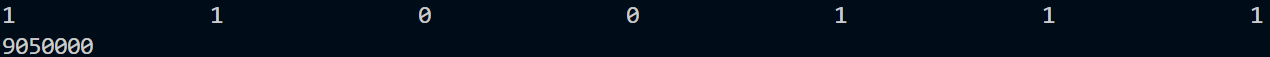
\includegraphics[width=\textwidth]{img/corrida4.png}
\end{figure}

\section{Discusión}
Debido a la restricción respecto al número de hormigas, para obtener la mayor rapidez y optimización posible, se dejó siempre el número de hormigas al máximo (7), los parámetros \emph{alpha} y \emph{beta} también debían tener cierto equilibrio para que el resultado fuera el mejor posible, finalmente, para asegurar que el algoritmo encontrara el mejor resultado posible (maximización), se estableció un número de iteraciones lo suficientemente grande (1000).

\section{Conclusión}
La elaboración de este proyecto deja en evidencia que es posible abstraer muchos problemas relacionados con la exploración y/o combinatoria para resolverlos con el algoritmo ACO, sin duda la principal herramienta de este algoritmo son los \emph{grafos}, por lo que cualquier problema que pueda representarse de esta forma podrá resolverse con ACO. Este algoritmo soluciona de una forma muy eficiente problemas de tipo \emph{NP}, sin embargo se requiere cierto grado de abstracción del problema, y existe cierto grado de \emph{randomness} que no es posible controlar.

\bibliographystyle{unsrt}
\bibliography{refs}
\nocite{*}

\end{document}
